\section{Monte Carlo Simulations}

First, we study the equilibrium properties by means of Monte Carlo simulations.

We start our simulations by selecting a particle at random, and attempting a translational and then a rotational move at that particle. Every consecutive step we select the first neighboring particle in the positive direction of $z$ axis.

In the translational move a particle is displaced along the z-axis ($z_{t+1} = z_t + \delta z$), where $\delta z$ is a random value uniformly distributed in the range $[+\eta, -\eta]$, with $\eta = 0.5 (\Delta z_{min} - \Delta z_0)$. Here $\Delta z_{min}$ is the interparticle distance for which the interaction energy between two aligned dipoles is minimal, and $\Delta z_0$ (shown as filled points at the Fig.~\ref{fig:interaction_energy}) is the interparticle distance for which the potential energy vanishes if we decrease distance starting from $\Delta z_{min}$.

For the rotational move a new orientation is chosen uniformly at random. A move is accepted with probability $\eta < \mathrm{min} \left\{1, \, \exp(\Delta E / k_BT) \right\}$, where $\eta$ is a random number uniformly-distributed in $[0, 1)$ and $\Delta E$ is the change in potential energy due to the trial move.

For the sake of simplicity, we restrict interactions to the first-neighbors.

We also consider periodic boundary conditions.

%\begin{figure}
%	\centering
%	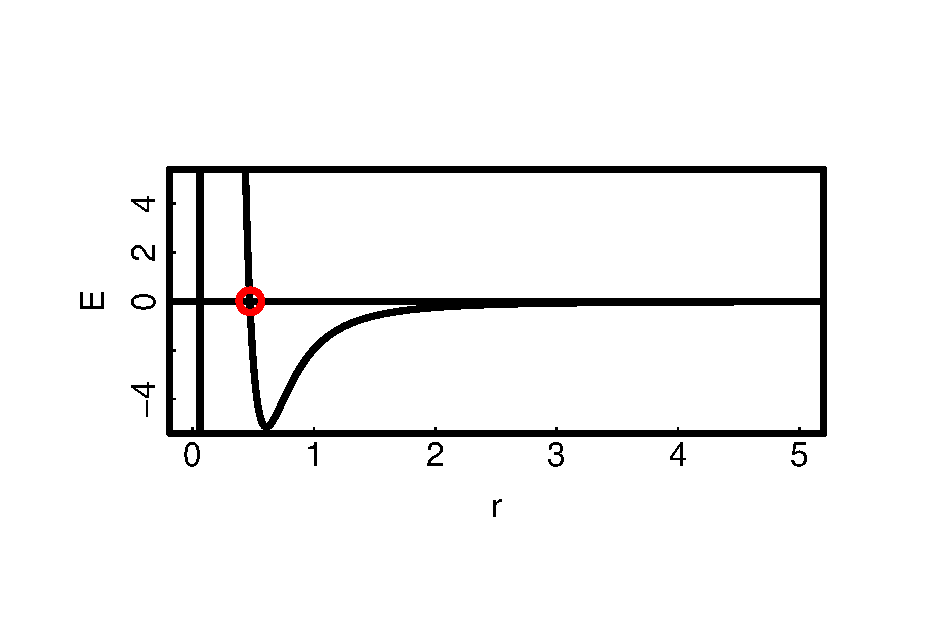
\includegraphics[width=0.6\textwidth]{Images/potential_energy_zero}
%	\captionsetup{justification=centering, width=0.9\textwidth}
%	\caption{Potential energy as function of interparticle distance for co-aligned configuration and $k = 10$, $A = 1000$. Red point shows location of $\Delta z_0$.}
%	\label{fig:delta_z_0_location}
%\end{figure}